\documentclass[10pt, a4paper]{report}

\usepackage[utf8]{inputenc}
\usepackage{polski}
\usepackage{a4wide}
\usepackage{fancyhdr}
\usepackage{lastpage}
\usepackage{tabularx}
\usepackage{graphicx}

\graphicspath{ {./img} }

%strona tytułowa
\begin{titlepage}

\title{\huge{\textbf{Sprawozdanie}}}
\author{Zespół 1}
\date{22.05.2022r}

\end{titlepage}

\renewcommand{\footrulewidth}{1pt}

\begin{document}
\maketitle

\renewcommand*\thesection{\arabic{section}} 

\pagestyle{fancy}
\fancyhf{}
\lhead{Sprawozdanie}
\rhead{Zespół 1}
\cfoot{Strona \thepage \hspace{1pt} z \pageref{LastPage}}

\fancypagestyle{plain}{
    \lhead{Sprawozdanie}
    \rhead{Zespół 1}
    \cfoot{Strona \thepage \hspace{1pt} z \pageref{LastPage}}
}
\tableofcontents
\newpage

\section{Skład zespołu}
Zespół składa się z 5 osób. Z racji faktu, że projekt jest prowadzony w metodyce zwinnej \textit{Scrum} nadaliśmy członkom zespołu odpowiednie role.

\begin{itemize}
    \item Adrian Nowosielski -- Product Owner, developer,
    \item Szymon Półtorak -- Scrum Master, developer,
    \item Cezary Skorupski -- developer,
    \item Michał Szlązak -- developer,
    \item Krystian Sereda -- developer.
\end{itemize}

\section{Temat Projektu}
Tematem naszego projektu jest \textit{Niezbędnik Edukacyjny}. Jest on narzędziem wspomagającym naukę oraz organizację czasu.
Zakładane są w nim następujące funkcje:
\begin{itemize}
    \item To Do -- lista zadań, które użytkownik będzie mógł sobie dodawać oraz sprawdzać, które zadania ukończył, a które są do zrobienia,
    \item Timer -- pozwala ustawiać interwały oraz stoper dla użytkownika,
    \item Calculator -- prosty kalkulator matematyczny pozwalający wykonywać proste obliczenia matematycznych,
    \item QuickNote -- moduł pozwalający wykonywać i zapisywać szybkie notatki.
\end{itemize}

\section{Środowisko powstawania projektu}
\begin{tabularx}{\textwidth}{ l|l } 
    \hline Nazwa & Wersja \\ 
    \hline IntelliJ Idea & 2022.1.1\\
    \hline Apache Maven & 3.8.1 \\ 
    \hline JavaFX & 18.0.1 \\
    \hline JUnit & 5.8.2\\
    \hline Java Development Kit & 17.03 LTS \\
    \hline
\end{tabularx}
\newpage

\section{Tablice sprintów}
W tym rozdziale pokazujemy zdjęcia z tablic w poszególnych sprintach.

\subsection{Sprint 1}
\begin{figure}[ht]
    \begin{center}
        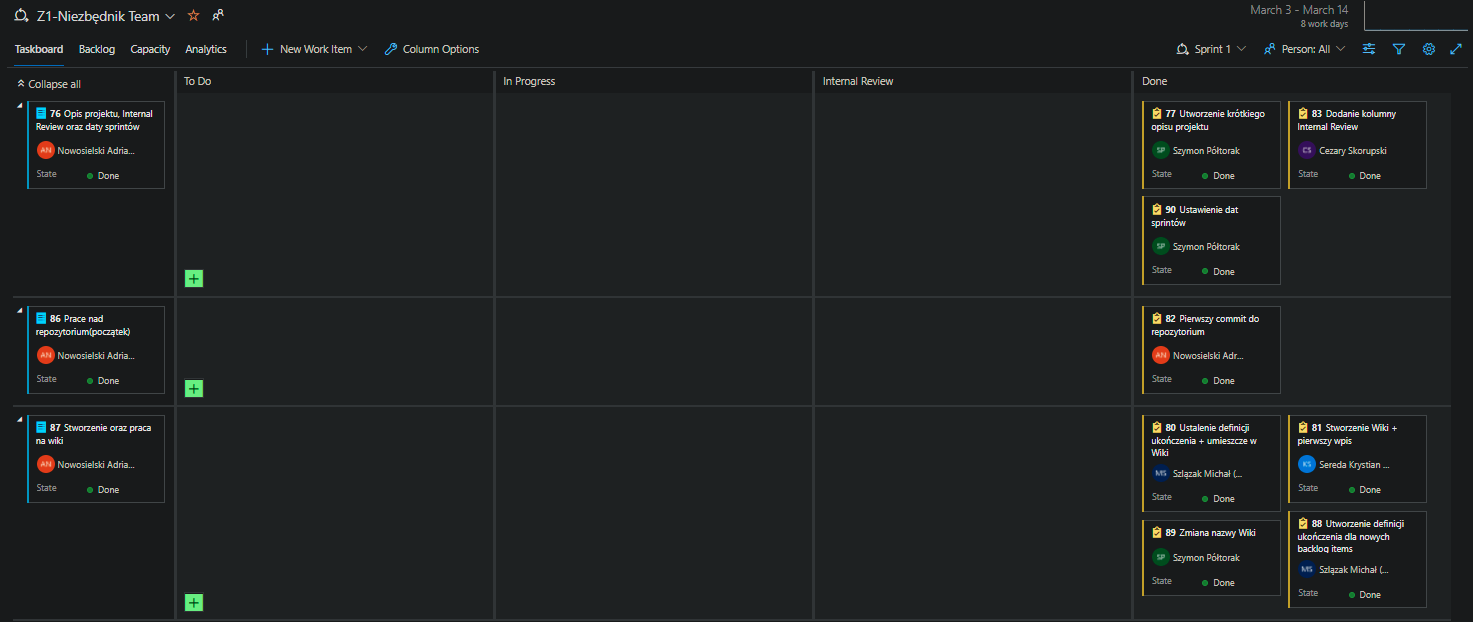
\includegraphics[scale=0.38]{s1.png}
        \caption{Sprint 1 tabela}
    \end{center}
\end{figure}
\newpage

\subsection{Sprint 2}
\begin{figure}[ht]
    \begin{center}
        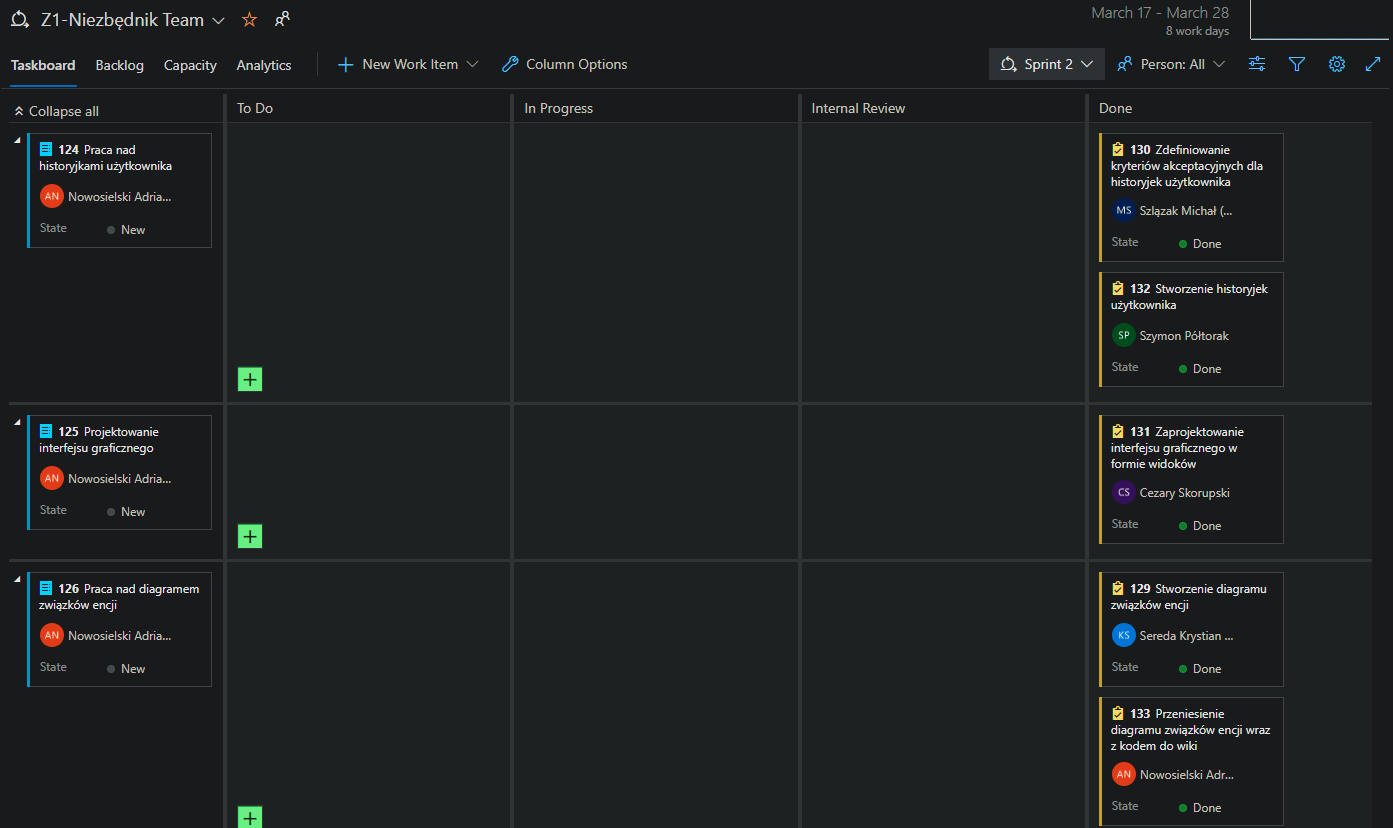
\includegraphics[scale=0.4]{s2.png}
        \caption{Sprint 2 tabela}
    \end{center}
\end{figure}
\newpage

\subsection{Sprint 3}
\begin{figure}[ht]
    \begin{center}
        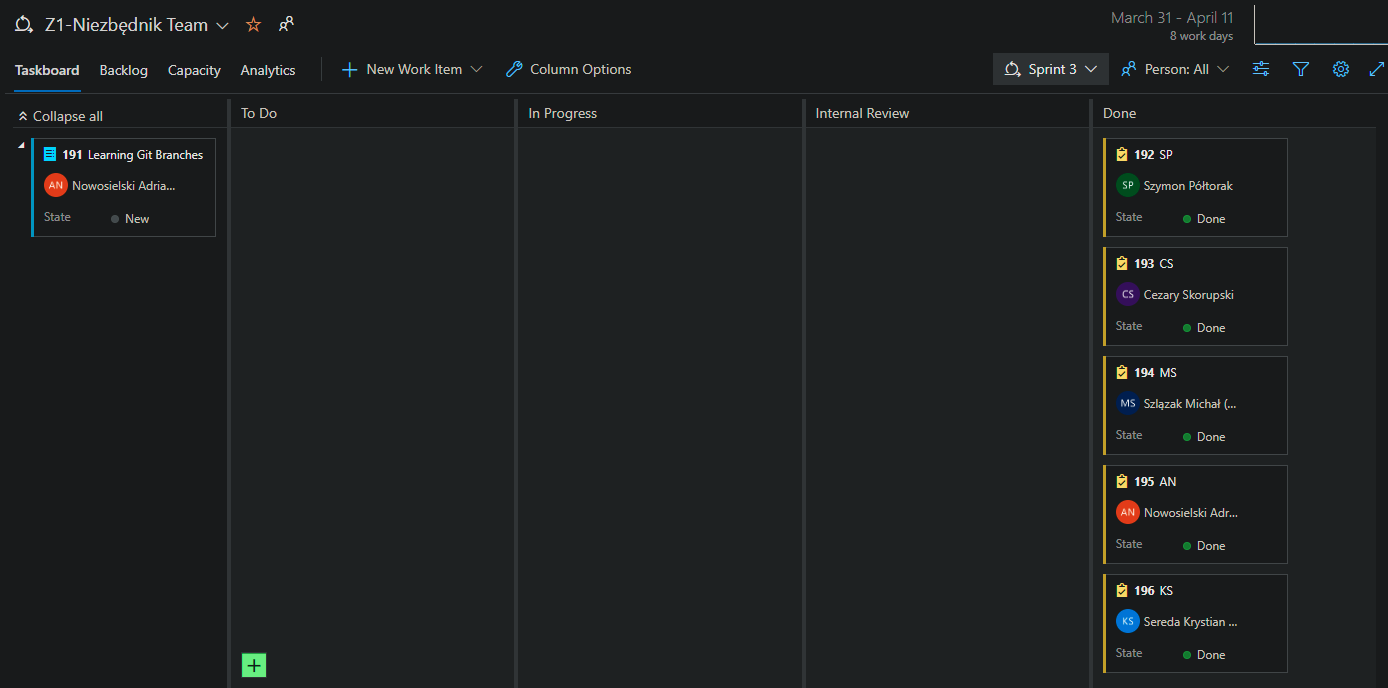
\includegraphics[scale=0.38]{s3.png}
        \caption{Sprint 3 tabela}
    \end{center}
\end{figure}

\subsection{Sprint 4}
\begin{figure}[ht]
    \begin{center}
        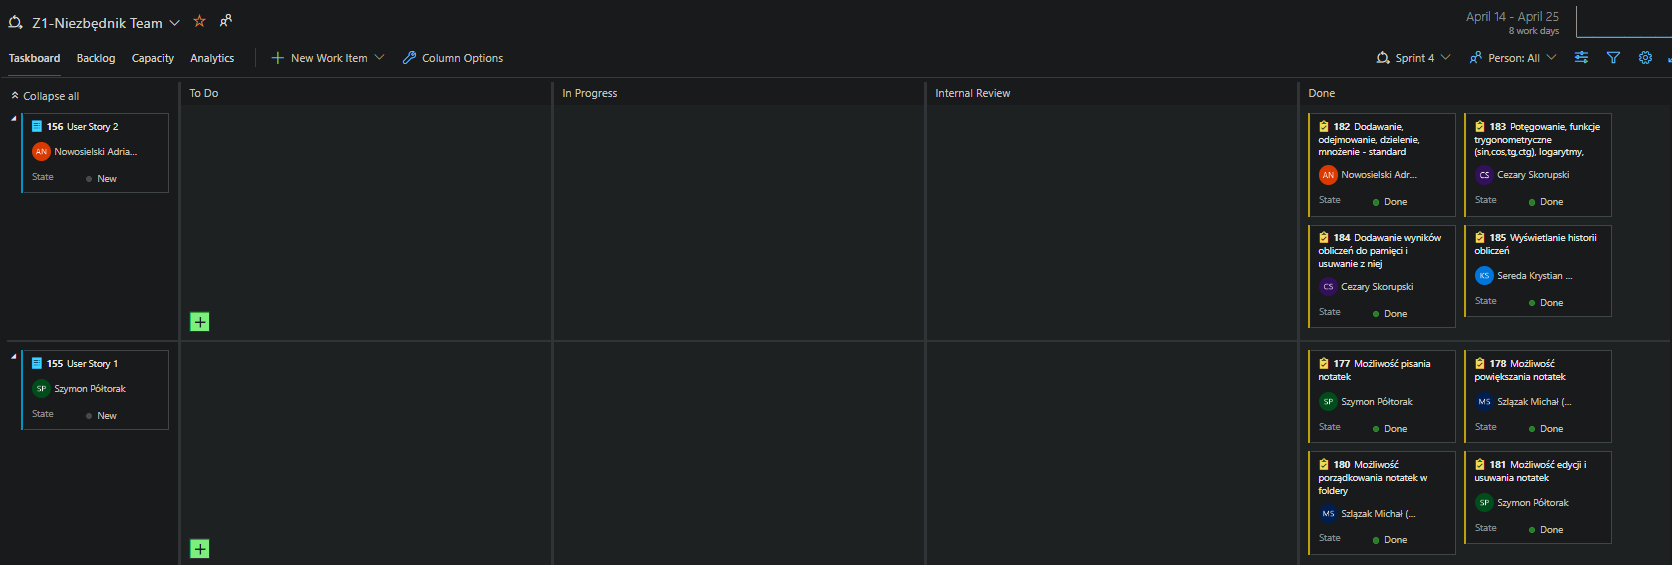
\includegraphics[scale=0.38]{s4.png}
        \caption{Sprint 4 tabela}
    \end{center}
\end{figure}
\newpage

\subsection{Sprint 5}
\begin{figure}[ht]
    \begin{center}
        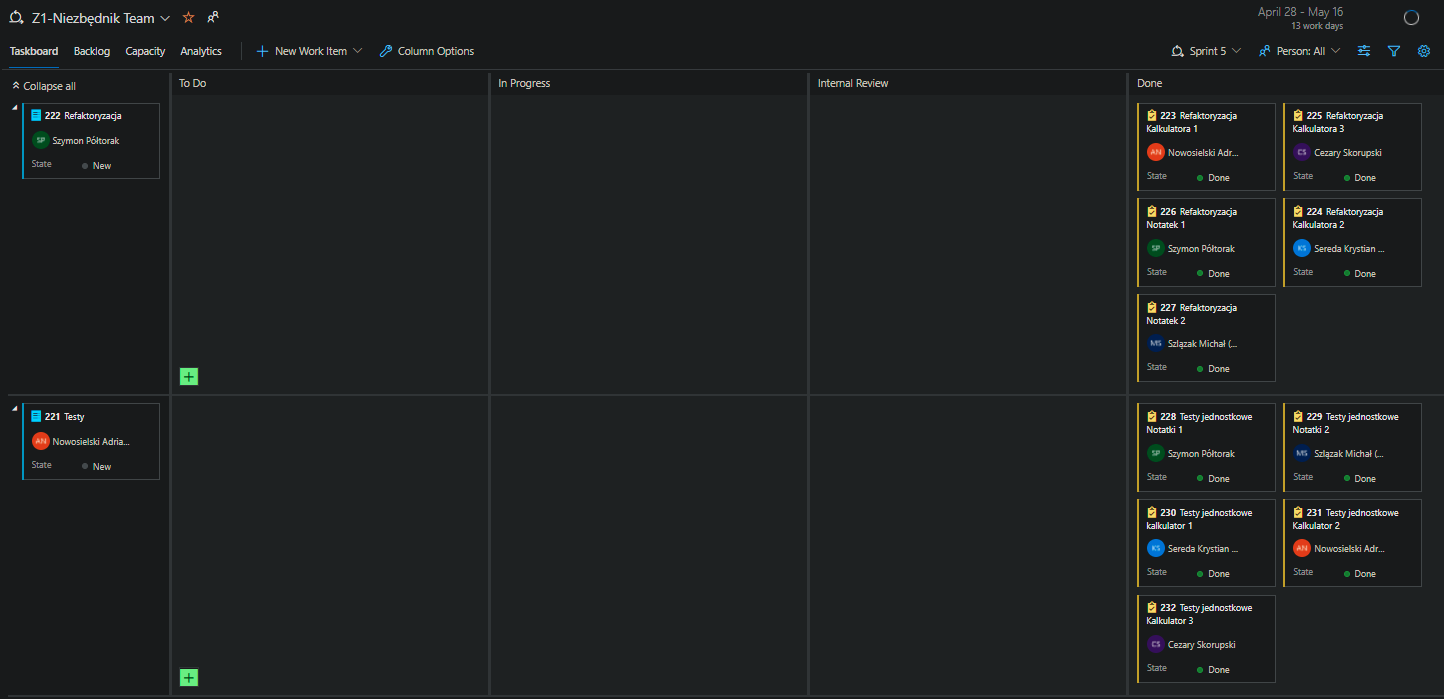
\includegraphics[scale=0.38]{s5.png}
        \caption{Sprint 5 tabela}
    \end{center}
\end{figure}
\newpage

\subsection{Sprint 6}
\begin{figure}[ht]
    \begin{center}
        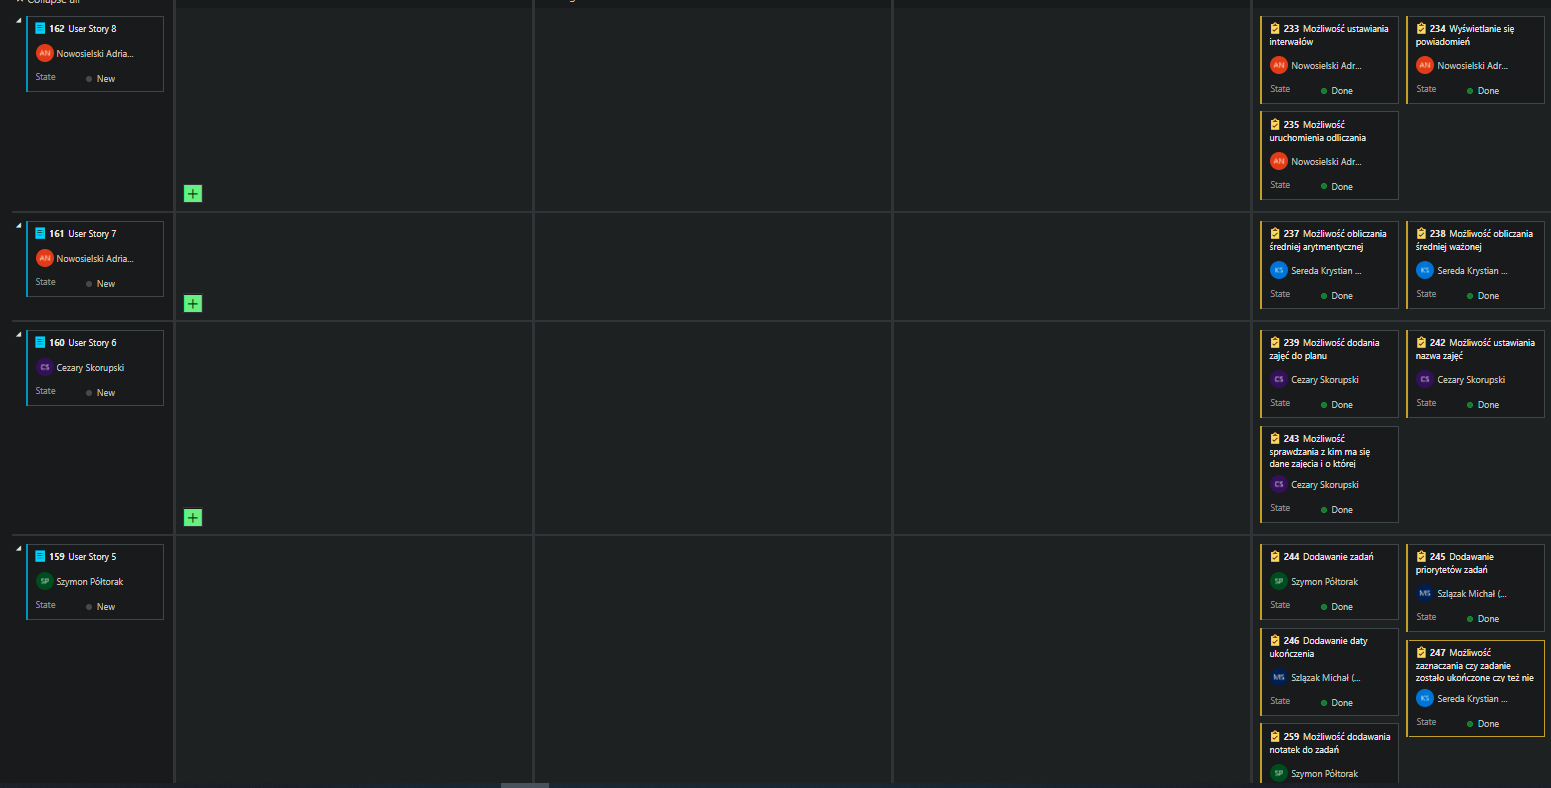
\includegraphics[scale=0.36]{s6.png}
        \caption{Sprint 6 tabela}
    \end{center}
\end{figure}

\section{Podsumowanie współpracy}
Organizacja pracy odbyła się za pośrednictwem platformy \textbf{Azure Dev Ops}. Komunikacja w~ zespole polegała 
na spotkaniach, organizowanych raz w tygodniu, na platformie \textbf{Microsoft Teams} oraz na komunikacji bezpośredniej w wiadomościach prywatnych
 na różnych komunikatorach internetowych.

\section{Podsumowanie Projektu}
Podczas trwania projektu udało nam się wykonać zdecydowaną większość zaplanowanych funkcjonalności.
Prace postępowały sprawnie dzięki odpowiedniej komunikacji oraz organizacji pracy. Niestety niektóre
zaplanowane przez nas funkcjonalności nie zostały wykonane z powodu liczby sprintów implementacyjnych oraz 
problemów jakie napotkaliśmy na początku tworzenia aplikacji. Spowodowane były one brakiem doświadczenia w pracy z
 technologiami jakie użyliśmy w projekcie. Z czasem jednak nauczyliśmy się z nimi pracować dzięki czemu podczas drugiego
 sprintu zespół był w stanie zrobić dwukrotnie więcej zadań niż podczas pierwszego sprintu implementacyjnego.
Aplikacja jest w pełni działającym produktem, spełniającym postanowione przez nas wymagania wobec jego kształtu.
Całość projektu była zrealizowana zgodnie z zasadami metodyki zwinnej \textbf{Scrum}.

\end{document}